\chapter{The Partial Derivative Matrix}\label{chap:evalDim}

In this chapter, we shall look at a powerful technique introduced by Nisan~\cite{nis91} that has been instrumental in many lower bound proofs and also in constructing polynomial identity tests.
Nisan~\cite{nis91} introduced the notion of the partial derivative matrix in the context of proving lower bounds for \emph{non-commutative} ABPs, and we shall see that first.

\section{Non-commutative models of computation}

A non-commutative polynomials over many variables, denoted by $\F\inbrace{x_1,\cdots, x_n}$, are formal polynomials over the variables wherein the variables do not commute.
Hence, a polynomial $x_1x_2 - x_2x_1$ in $\F\set{x_1,\cdots, x_n}$ is a non-zero polynomial.
They naturally can be added or multiplied but the order in which the variables are multiplied become important.
Hence,
\[
(x_1 + x_2)(x_1 + x_2) \spaced{=} x_1^2 + x_2x_1 + x_1x_2 + x_2^2 \spaced{\neq} x_1^2 + 2x_1x_2 + x_2^2
\]
Each monomial is no longer identifiable by just an exponent vector but is rather a \emph{word} on the set $\set{x_1,\cdots, x_n}$. 

In this space, we can continue to talk about arithmetic circuits or algebraic branching programs where we always keep track of the order of variables multiplied.
In arithmetic circuits or formulas, every $\times$ gate has labelled left and right children.
In an algebraic branching program, the weight of a path from source to sink is the product of the edge weights \emph{in the order from left to right}.

Nisan \cite{nis91} asked the question of whether we can prove lower bounds in this more restricted model of computation. In his paper, he introduced the complexity measure via the \emph{Partial Derivative Matrix}, and used it to not just prove lower bounds but exactly calculate the size of the smallest non-commutative ABP computing a homogeneous polynomial $f$. \\

\begin{exercise}
Show that, given any non-commutative ABP of size $s$ computing a homogeneous non-commutative polynomial of degree $d$, we can construct a homogeneous non-commutative ABP (edge weights are homogeneous linear forms) of size at most $s \cdot \poly(d)$ computing $f$. 
\end{exercise}

\subsection{Partial derivative matrix for non-commutative ABPs}

\begin{definition}[Nisan's partial derivative matrix \cite{nis91}] Let $f$ be an $n$-variate homogeneous non-commutative polynomial of degree $d$. For any $i \in [d]$, the matrix $M_i(f)$ is defined follows:
  \begin{quote}
    The matrix $M_i(f)$ has $n^i$ rows and $n^{d-i}$ columns, indexed by monomials (or words) of length $i$ and $d-i$ respectively. The entry at $(m_1, m_2)$ is the coefficient of the monomial (or word) $m_1 \cdot m_2$ in $f$. \qedhere
  \end{quote}
\end{definition}

\begin{theorem}[\cite{nis91}]\label{thm:nis-noncomm-abp}
For any $n$-variate homogeneous non-commutative polynomial $f$ of degree $d$, the smallest non-commutative ABP that computes $f$ must have size
\[
\rank(M_0(f)) + \rank(M_1(f)) +  \cdots + \rank(M_{d-1}(f)).
\]
\end{theorem}
The above is not an estimate; Nisan's result says that the sum of the ranks of the partial derivative matrix is \emph{exactly} the size of the smallest ABP.
The proof of this theorem is not hard, especially once you know what the answer is.
We shall prove part of the proof to show that the sum of the ranks is a lower bound for the size of the smallest ABP, and leave the other direction as an exercise.

\begin{proof}
Let $C$ be the smallest non-commutative ABP computing the polynomial $f$. We shall show that number of vertices in layer $i$ is at least the rank of $M_i(f)$. 

Suppose $v_1,\cdots, v_r$ are the vertices in the $i$-th layer, and let $s$ be the unique source node and let $t$ be the unique sink node.
For each $i \in [r]$, let $g_i$ be the non-commutative polynomial computed by the restricted ABP if we consider $s$ as the source and $v_i$ as the sink.
Similarly, let $h_i$ be the non-commutative polynomial computed by the restricted ABP with $v_i$ as source and $t$ as the sink.
Then, $f = g_1 h_1 + \cdots + g_r h_r$.
Since the ABP is homogeneous, each $g_i$ is a homogeneous non-commutative polynomial of degree $i$ and each $h_i$ is a homogeneous non-commutative polynomial of degree $d-i$.
Now consider the matrix the $n^i \times r$ matrix $G$, with rows indexed by monomials (or words) of degree $i$ and columns indexed by $[r]$, with the $(m,i)$ entry being the coefficient of $m$ in $g_i$.
Similarly, let $H$ be the $r \times n^{d-i}$ matrix, with rows indexed by $[r]$ and columns indexed by monomials (or words) of degree $d-i$, with the $(j,m)$ entry being the coefficient of $m$ in $g_j$.
\begin{subclaim}\label{subclaim:Nisan-ABP-proof}
$M_i = G \cdot H$. 
\end{subclaim}
\noindent 
With this claim, it follows that the rank of $M$ is a lower bound for $r$. 
\end{proof}

\begin{exercise}
Complete the proof of  \autoref{subclaim:Nisan-ABP-proof}, and also show that the bound is tight to show the other direction of \autoref{thm:nis-noncomm-abp}. 
\end{exercise}

\subsection{An explicit hard polynomial}

To complete the proof, we just need to construct an explicit polynomial for which one of the $M_i$'s has large rank.
A natural attempt is to make $M_{d/2}$ to be full-rank by making it something like the identity matrix.
Indeed, if we choose the polynomial to be the \emph{double polynomial} $\mathrm{Doub}_d$ defined as
\[
\mathrm{Doub}_d \spaced{:=} \sum_{w\in \set{x_1, \cdots, x_n}^{d/2}} \vecx_{w} \vecx_w
\]
or the \emph{Palindrome polynomial} $\mathrm{Pal}_d$ defined as
\[
\mathrm{Pal}_d \spaced{:=} \sum_{w\in \set{x_1, \cdots, x_n}^{d/2}} \vecx_{w} \vecx_{\mathrm{reverse}(w)},
\]
then clearly $\rank(M_{d/2})$ is $n^{d/2}$ giving the required lower bound. 

\begin{theorem}[\cite{nis91}] Any non-commutative ABP computing the polynomial $\mathrm{Doub}_d$ or $\mathrm{Pal}_d$ must have size $n^{\Omega(d)}$. 
\end{theorem}

As an added bonus, it is easy to see that $\mathrm{Pal}_d$ can in fact be computed by a non-commutative circuit of size $\poly(n,d)$.
Thus, this in fact yields an exponential separation between non-commutative ABPs and non-commutative circuits.
 
An important point to also observe is that this lower bound implies that an analogue of the depth reduction of \cite{vsbr83} is simply not possible in the non-commutative world. 

\section{Applications in the commutative world}

There are some instances in the commutative world where computation behaves like a non-commutative computation.
An example of this is the class of what are called \emph{read-once oblivious algebraic branching programs (ROABP)}, first defined by Forbes and Shpilka~\cite{FS13}. 


\begin{definition}[Read-once oblivious algebraic branching programs (ROABP) \cite{FS13}]
An ABP (over commuting variables) is said to be an \emph{read-once oblivious algebraic branching program (ROABP) in the order $(x_1,\cdots, x_n)$} if it has the property that all edge weights between layer $i$ and layer $i+1$ are \emph{univariate polynomials} in $x_i$.
\end{definition}


As seen in \autoref{chap:notation}, if $f$ is computable by an ROABP of width $w$,  then $f$ can be equivalently expressed as one entry of an iterated product of \emph{univariate} matrices.
That is,
\[
f \spaced{=} \inparen{A_{1}(x_1) \cdots A_n(x_n)}_{(1,1)}
\]
where each $A_i(x_i)$ is a $w\times w$ matrix (where $w$ is the width of the ABP) with entries as univariate polynomials in $x_i$. 

In some sense, this is essentially a non-commutative computation that is masquerading as a commutative computation since the variables are multiplied in the same order.
Thus, the partial derivative matrix that was used in the non-commutative ABP lower bound can also be used here.
We shall abuse notation and use the following definition of the partial derivative matrix that is more useful for the commutative world.

\begin{definition}[Partial derivative matrix for a partition] \label{defn:pdm-commutative}
For any given partition of variables $X = Y \sqcup Z$, define the \emph{partial derivative matrix} $M_{Y,Z}(f)$ to be the matrix described as follows --- the rows are indexed by monomials in $Y$, columns indexed by monomials in $Z$, and the $(i,j)$-th entry of the matrix is the coefficient of the monomial $m_i(Y)\cdot m_j(Z)$ in $f$. 
Further, we shall call a polynomial $f$ to be \emph{full-rank} if $M_{Y,Z}(f)$ is full-rank.
\end{definition}

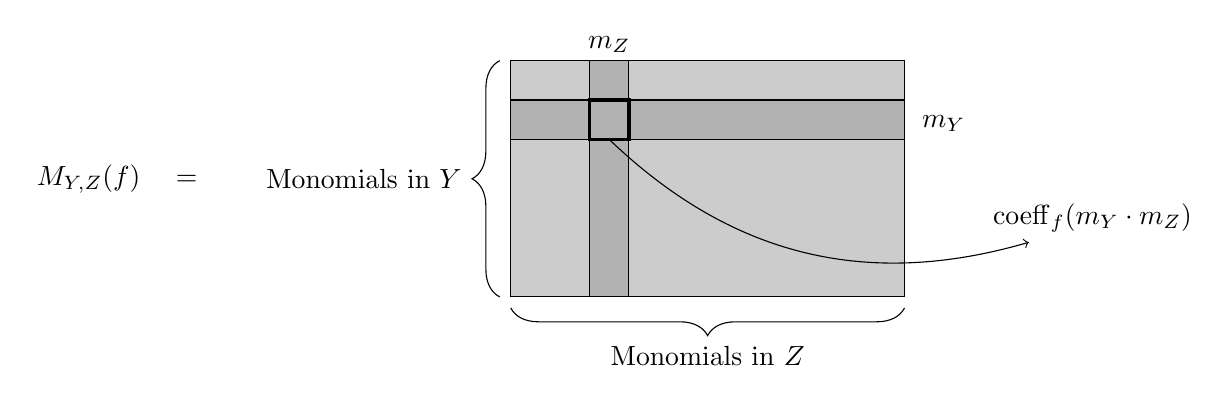
\begin{tikzpicture}
\node at (-5,1.5) {$M_{Y,Z}(f) \quad= $};
\draw[fill=black!20] (0,0) rectangle (5,3);

\draw[decorate,decoration={brace,amplitude=10pt,raise=4pt},yshift=0pt]
(0,0) -- (0,3);
\node[anchor=east] at (-0.5,1.5) {Monomials in $Y$};
\draw[decorate,decoration={brace,amplitude=10pt,mirror, raise=4pt},yshift=0pt] 
(0,0) -- (5,0);
\node[anchor=north] at (2.5,-0.5) {Monomials in $Z$};

\draw[fill=black!30] (1,0) rectangle (1.5,3);
\node at (1.25,3.2) {$m_Z$};

\draw[fill=black!30] (0,2) rectangle (5,2.5);
\node at (5.5,2.2) {$m_Y$};

\draw[very thick] (1,2) rectangle (1.5,2.5);

\node[anchor=west] at (6,1) {$\mathrm{coeff}_f(m_Y \cdot m_Z)$}
edge[<-,bend left] (1.25,2);
\end{tikzpicture}

\medskip

\noindent
The following observation is a an easy exercise. 

\begin{lemma}
Suppose a polynomial $f$ is can be computed as an entry in a product of $w\times w$ univariates matrices in the order $(x_1,\cdots, x_n)$, that is
\[
f \spaced{=} \inparen{A_1(x_1) \cdots A_n(x_n) }_{(1,1)}.
\]
Then, for every $i \in [n]$, for the partition $Y = \set{x_1, \ldots , x_{i}}$ and $Z = X \setminus Y$ we have $\rank(M_{Y,Z}(f)) \leq w$. 

Furthermore, the converse also holds. 
\end{lemma}

Hence, the rank of the partial derivative matrix can be used to prove lower bounds for ROABPs. \\

\begin{exercise}\label{ex:pdm-rank}
What is the rank of the partial derivative matrices for the following polynomials? 
\begin{itemize}
\item The elementary symmetric polynomials $\ESym_d$, under any partition.
\item Any $\SES$ circuit of size $s$, under any partition.
\item $\Det_n$ and $\Perm_n$ under the partition $X = Y \sqcup Z$ where $Y$ the variables from the first $n/2$ rows. 
\item The polynomial $(x_1 + x_2) \cdots (x_{2n-1} + x_{2n})$ under the partition $X = Y \sqcup Z$ with $Y = \set{x_1,\cdots, x_n}$. 
\item The polynomial $(x_1 + x_2) \cdots (x_{2n-1} + x_{2n})$ under the partition $X = Y \sqcup Z$ with $Y = \set{x_1,x_3,x_5,\cdots, x_{2n-1}}$. 
\end{itemize}
\end{exercise}

\subsection{An evaluation perspective}

For this section, let us assume that we are working with a field that is large enough. The following is an alternative way to study the rank of the partial derivative matrix under some partition. It is essentially the same, but sometimes is easier to reason with and we shall see a few examples in this chapter. 

\begin{definition}[Evaluation dimension]
Let $X = Y \sqcup Z$. The evaluation dimension of a polynomial $f$, with respect to $Y \sqcup Z$, denoted by $\evalDim_{Y,Z}(f)$,  is defined as the rank of the following polynomials
\[
\evalDim_{Y,Z}(f) \spaced{=} \rank\inparen{\setdef{f(\veca, Z) \in \F[Z]}{\veca \in \F^{|Y|}}}. 
\]
In other words, $\evalDim_{Y,Z}(f)$ of the space of partial evaluations of $f$ by setting $Y$ to arbitrary field constants. 
\end{definition}

\noindent 
The following lemma is easy to verify.

\begin{lemma}\label{lem:evalDim-to-coeffDim}
Over any field $\F$, we always have that $\evalDim_{Y,Z}(f) \leq \rank(M_{Y,Z}(f))$. If $|\F| \geq \deg(f)$, then
\[
\evalDim_{Y,Z}(f) \spaced{=} \rank(M_{Y,Z}(f)).
\]
\end{lemma}

To illustrate why this perspective is convenient, we shall take one example from \autoref{ex:pdm-rank} and compute the evaluation dimension of a $\SES$ circuit. 

\begin{claim}
Let $f = \sum_{i=1}^s \ell_i^d$. Then under any partition $X = Y \sqcup Z$, we have that $\evalDim_{Y,Z}(f) \leq (d+1) \cdot s$. 
\end{claim}
\begin{proof}
  It suffices to prove that the evaluation dimension of a single $\ell^d$ is at most $(d+1)$ and the lemma would follow due to sub-additivity.
Say $\ell = (a_0 + a_1 x_1 + \cdots + a_nx_n)$.
For any partition $X = Y \sqcup Z$, let $\ell_Y = \sum_{i\in Y} a_i x_i$ and $\ell_Z = \ell - \ell_Y$ so that $\ell = \ell_Y + \ell_Z$. Now if we take a partial evaluation of the $Y$ variables to field constants, the resulting polynomial is 
\[
(\alpha + \ell_Z)^d \spaced{=} \alpha^d \;+\; \alpha^{d-1} \binom{d}{1} \ell_Z \;+\; \cdots \;+\; \ell_Z^d. 
\]
And as we change the evaluation, the only change in the above equation is the value of $\alpha$. Hence it is clear that the rank of this space of polynomials is no more than $(d+1)$ as it is spanned by 
\[
\set{1, \ell_Z, \cdots, \ell_Z^d}.\qedhere
\]
\end{proof}

\begin{exercise}
Repeat \autoref{ex:pdm-rank} with evaluation dimension. 
\end{exercise}

\begin{exercise}
Suppose you have a degree $d$ polynomial $f$ so that $\dim{\partial^{\leq d}(f)}$ is at most $r$, that is, there are at most $r$ linearly independent partial derivatives of $f$. What can you say about $\evalDim_{Y,Z}(f)$ under any partition? 

What about the converse?
\end{exercise}

\bigskip 

The notion of partial derivative matrix is very useful and in the next chapter we shall see how it can be used to prove lower bounds for multilinear models.

%%% Local Variables: 
%%% mode: latex
%%% TeX-master: "fancymain"
%%% End: 
